\documentclass[a4paper,10pt]{report}
\usepackage[utf8x]{inputenc}
\usepackage{url}

\usepackage{titling}
\usepackage{amsmath}
\usepackage{amssymb}
\usepackage{graphicx}
\usepackage{listings}
\usepackage{caption}
\usepackage{subcaption}

\bibliographystyle{vancouver.bst}

% Title Page
\pretitle{\begin{center}\Huge CS344 - Final Report \end{center}\begin{center}}
\title{\Huge Smart Phone Cryptography}
\posttitle{\end{center}\begin{center}\LARGE A comparison of techniques for encrypted data communication \end{center}}


\preauthor{\begin{center}\LARGE Tom Nicholls - 1006007\end{center}\begin{center}}
\author{Discrete Mathematics - Year 3}
\postauthor{\end{center}\begin{center}\large Marcin Jurdzinski\end{center}}

\begin{document}
\maketitle

\begin{abstract}
%Should be 200 words - check before final proof read

Protecting sensitive or secret information has always been an important issue. With the increased popularity and usability of smartphones, tasks from accessing confidential work files or personal bank accounts to communicating with clients and friends, are being completed through applications over mobile or wireless internet connections. In this project the various cryptographic schemes used by popular applications available to Android based smartphones for secure data communication will be researched. Accompanying this will be a study of other cryptographic schemes. These techniques will be implemented through a data transmission application. Tests will be carried out to analyse various important factors that need to be considered for a successful encrypted data transmission application. An original conclusion will then be drawn as to whether the current techniques of cryptography available are appropriate or if a new scheme should be encouraged. The results of the described implementation and analysis were that the currently used cryptographic techniques are appropriate for the current state of smartphone usage and capabilities. These techniques, however, should be combined to create a new application. A different technique, which has increased security for a smaller resource cost, exists that can easily be used in the event that the requirements of the current cryptographic schemes surpass the available resources of current smartphones. 

{\bf Keywords:} Cryptography, Encryption, Decryption, Smartphone, Android, AES, RSA, ECC
\end{abstract}

\tableofcontents


\chapter{Introduction}


\section{Background}

To start this project report, all relevant background information will be presented allowing the reader to fully understand all aspects of the project. An overview of basic techniques and topics will be given, with a greater explanation for more specialised areas. 

\subsection{Smartphones}

In this section, the basics of the smartphone will be introduced and described. As smartphones are a prominent part of modern culture, and therefore known in some degree to everybody, only an overview will be given. The book by Sarah Allen et al. \cite{whatisasmartphone} was used as reference material.

'Mobile' or 'Cell' phones have been available for commercial use since the beginning of the 1980s. The most popular functions of these phones are for telephone calls, text or multi-media message sending or even basic internet access and games. With the development of the smartphone these older devices are considered low-end phones. Higher-end phones, universally named the 'smartphone' provide the same basic features (telephone calls, messaging etc) but with a plethora of added functions such as full internet access, as well as increased computing capabilities through more powerful processors and other hardware. Smartphones also utilise the QWERTY keyboard and a larger, higher-resolution, screen. 

Compared to desktop computers, smartphones have a diverse set of operating systems, determined by the manufacturer of the smartphone. Smartphone operating systems include; Apple iPhone iOS \cite{appleios}, Windows Phone \cite{windowsphone} and Google Android \cite{googleandroid}. Each operating system, unlike that of a desktop, determines which programming language a developer must use if they are to develop an app for a particular smartphone. This leads to a separate application marketplace, a database where users can download and install new applications, for each smartphone operating system. Whilst applications can be developed in a cross-platform manner, through the use of HTML and CSS, this is not yet standard, so the various marketplaces are individual in the applications that are on offer. The Android operating system, developed by Google and mostly found on devices by Samsung, HTC or Google themselves, use the Google Play marketplace \cite{googleplay} for application distribution with applications being developed using the Java programming language.

The message sending capabilities of smartphones is the feature that is most important for this project, whether it be using the in-built short messaging service (SMS) or through the use of an installed application. Message sending allows the specification of a recipient and a user entered message for that recipient, with a near instant sending and receiving of that message. On average, the message is of a short length and can be described as an easier, more lightweight form of simple email exchange. 

\subsection{Cryptography}

Taken from the book by Richard A. Mollin \cite{richardmollin}, the meaning of cryptography is 'the study of methods for sending messages in secret (namely, in enciphered or disguised form) so that only the intended recipient can remove the disguise and read the message (or decipher it).' Many keywords are used in the study of cryptography and help to give an introduction to the field; 

\begin{itemize}
 \item Plaintext - The original message, input by the initiating user.
 \item Ciphertext - The disguised message, created using the plaintext.
 \item Encryption - The process of transforming the plaintext into the ciphertext.
 \item Decryption - The process of turning the ciphertext into the original plaintext. Accomplished by the recipient, who has the knowledge to remove the disguise.
 \item Cipher - The Method for enciphering and deciphering.
 \item Cryptanalysis - The study of mathematical techniques for attempting to break the cryptographic methods.
 \item Cryptographic Key - A tool for encryption or decryption
\end{itemize}

\noindent
This shows that basic cryptography has the following form:

\begin{center}

  \textbf{Plaintext} $\rightarrow$ \emph{Encryption} $\rightsquigarrow$ \textbf{Ciphertext} $\rightsquigarrow$ \emph{Decryption} $\rightarrow$ \textbf{Plaintext}

\end{center}

\noindent
Two very basic examples of cryptography, which can and have been expanded into many different, more elaborate, techniques, are the substitution and transposition ciphers. Substitution ciphers replace symbols in the plaintext with other symbols, using a given rule (the key), to produce the ciphertext. For example, the key may be; a $\rightarrow$ q, b $\rightarrow$  f, c $\rightarrow$  m, and so on. A transposition cipher, on the other hand, transposes the places in which the plaintext letters are situated. This means that no new letters are introduced. The key for this cipher is a permutation that describes how the letters should be transposed. For a plaintext that consists of 10 letters, the key could be:

\begin{center}
$
\begin{pmatrix}
  1 & 2 & 3 & 4 & 5 & 6 & 7 & 8 & 9 & 10 \\
  1 & 2 & 5 & 7 & 6 & 4 & 9 & 10 & 3 & 8
 \end{pmatrix}
$
\end{center}

where the symbol in the position number in the top row, is replaced by the symbol in the position number below it (in the second row). Using these techniques as a basis, other more advanced cryptographic schemes can be created and are defined by the cipher (and key) that is used for the particular method.

Cryptography has been used in some form or another to exchange secret message throughout history. For example, the first use of of cryptography in a military setting was by the Spartans in 475 B.C. In the modern age, cryptography is most commonly used when sending or storing data using a computer system, such as sending an email across a network, or saving a file on a company server. 

\section{Motivation}

Protecting important and secret information is big issue, particularly when data such as bank accounts details or private work related conversations are taking place or being exchanged. When new devices or computer systems are developed and deployed, the security of that system is always considered and studied. Smartphones, on the other hand, have a substantial amount of user-input in the form of publicly developed applications. With smartphones becoming the most popular tool for communicating and completing other tasks with the transfer of sensitive information combined with the fact that there are a vast number of tools for completing such tasks, the study of the strength and current state of security of smartphones is an ever evolving field. This creates a number of questions, the answers to which form the basis of this project:

\begin{itemize}
 \item Do applications that facilitate the secure transfer of messages exist?
 \item What are the cryptographic techniques behind these applications?
 \item Are there other techniques which could also be used for this purpose?
 \item What is the performance of these styles applications?
 \item Can these applications or methods be improved upon?
 \item Can a conclusion be made about the current state of secure message communication and its future? 
\end{itemize}

The results of this project will contribute an original conclusion to the field of cryptography within smartphones. Preliminary research showed that the questions set out to be answered in this project have not been answered before for the current, present-day state of smartphones. This is important because even in the last few years significant improvements and developments have been made concerning the design and processing power of smartphones which has had a tremendous affect on smartphone usability, for example the more advanced and widely available use of GPS in direction planning. 

\section{Scope and Limitations}

It is important to set out in the introduction to this project report what the scope of the project is and to describe any limitations that have been placed on the project.

Firstly, as will be detailed later in this report, the choice was made that any developed software will be in the Java programming language and that the Android operating system will be the focus of study and application development. This is so that the project can be accomplished within the given time frame, to the standard required and with the hardware that is more easily available. It also ensures that the project does to try to encompass an area that is so huge that any conclusion loses focus and therefore its value.

This project also focuses on the use of cryptography in sending secure messages between users as opposed to other issues regarding smartphone security. A few examples of other forms of security related to smartphones could be a study of stored data protection, techniques to retrieve data from a smartphone wirelessly and protecting a smartphone from attacks or viruses. The reasons that this project is focused on one particular aspect of security with smartphones is much that same as the reasons given for the previous point. Furthermore, narrowing the scope of the project in this way means that a full solution and conclusion can be found for this particular aspect, as opposed to giving brief or vague conclusions for a number of aspects. Cryptography, particularly in this setting, also allows for a project that encompasses both computer science and mathematics and therefore is appropriate for a Discrete Mathematics student. 

Lastly, this goal of this project is not to design and develop a product (application) that meets industry and user requires and can be sold or released to the general public. A project of that type would focus more on human-computer interactions, product design and marketing, as opposed to focusing on the mathematically based computer science areas of smartphones and cryptography. Therefore, the project can be categorised as a combination of both a research based and software development based project, each emphasising and reinforcing the other. 

\section{Issues}

Every project is faced with issues regarding the projects final goals and outcomes, or the techniques or methods used to reach these outcomes. This section will discuss the issues faced or considered with this project. 

\subsection{Legal}

Legal issues are the main issues that need to be considered with this project. As a large section of this project is research based, it needs to be ensured that all materials used are correctly and appropriately referenced. Furthermore, as this project is centred on the issues of computer security, in the form of cryptography, legal issues need to be discussed \cite{dataprotect} \cite{internetlaw}. As long as any material that is encrypted is legal in its own rights and that only data that is solely owned by myself is used in the cryptographic processes, then any legal issues will be avoided in this case. Also, the resulting product facilitates the secure communication of messages which, in the wrong hands, could be used to aid a number of illegal operations. To avoid the direct use of the final application for illegal purposes, it will not be published to the Google Play application marketplace and will therefore not be available to the public. This also means that a disclaimer or end-user license agreement (EULA) will not be required, which would included the consultation of a professional lawyer. If the software created in this project was obtained by a malicious user, then any data required by the police could and would be given to break the illegal encryption by the author \cite{pcworldart}.

\subsection{Ethical}

In almost all modern technical advances, ethical issues can be found, posing unique problems depending on the perception or views of the topic by various groups or persons. For this topic, the legal issues presented above can also be viewed as ethical issues. Should an application be developed, or a field be advanced, that could be used to facilitate illegal operations? This question, and many like it, could and are constantly discussed and argued by professionals and amateurs alike, from almost all academic backgrounds. Because of this, a universally agreed upon set of ethics will never be concretely reached. However, through the actions taken to escape any legal issues, the avoidance of any major ethical issues are avoided. 

As no interviews, questionnaires or experiments will be taken place in this project, other ethical issues regarding this do not need to be considered. 

\subsection{Social and Professional}

With smartphones and text messaging services already being a central part of society, this project does not face any social issues. %not really sure where to go from here or what to talk about for professional issues

\section{Report Structure}

The structure of the report from this point onwards will be as follows:

\begin{description}
  \item[Objectives] A discussion of the objectives and goals of the project.
  \item[Research] Presentation and thorough explanation of all research completed.
  \item[Design] Full system design, outlining and explaining choices made and tools used. 
  \item[Development] Implementation and software development aspect of the project presented, including the testing phase.
  \item[Results] Analysis of the developed system accompanied with all conclusions and results found. 
  \item[Further Work] All further work completed for this project and a suggestion and discussion of any improvements that could be made.
  \item[Project Conclusion] A conclusion of the project as a whole, including self-assessment.
  \item[Acknowledgements] A list of acknowledgements relating to this project.
  \item[References] All reference material used through the project.
\end{description}

Theorems, proofs, code snippets, diagrams and screen shots will be used throughout, as required, to improve understanding and to help explain various sections of this report. 


\chapter{Objectives} %Could be expanded upon???

In order to answer the questions described previously, certain goals and objectives must be met. The main objectives of this project where: 

\begin{enumerate}
  \item Research
  \begin{itemize}
    \item Framework design
    \item Currently Available Applications
    \item Cryptographic Techniques
    \item Relevant factors that can be used to compare schemes implemented on a mobile device
  \end{itemize}
  \item Development
  \begin{itemize}
    \item Framework
    \begin{itemize} 
      \item Design Data Communication framework
      \begin{itemize}
        \item Server
        \item Mobile Application
        \item P.C Client
      \end{itemize}
    \end{itemize}
  \item Encrypted Data Communication
  \begin{itemize}
    \item Design and implement cryptographic techniques
  \end{itemize}
  \end{itemize}
  \item Analysis
  \begin{itemize}
    \item Perform tests from research
    \item Collect and present results
  \end{itemize}
  \item Conclusion
  \begin{itemize}
    \item Present and justify the findings and conclusions that can be made form the completed tests
    \item Show possible adjustments to the implemented schemes which would increase their usability
  \end{itemize}
  \item Further Work
  \begin{itemize}
    \item Detail possible extensions that can be made to the systems to include other possible functions
  \end{itemize}
\end{enumerate}

All aspects of software development are accompanied by thorough testing and are completed using a test driven development technique in a plan-driven setting, as described by Ian Sommerville \cite{iansommerville}. A further breakdown of the objectives, together with a thorough project task timetable, can be found in the form of a Gantt chart in Appendix \ref{A}.

\chapter{Research}

All completed research will now be presented, corresponding with the goals included in the Objectives section of this report. 

\section{Framework}

The system framework refers to the developed software that will facilitate the communication of data messages between any two users of the system, whilst not including any form of encryption or decryption. The research required to design a system framework was fairly minimal as most aspects of the software development for this project has already been covered, however how a full system should be set up had not. As the Java programming language had already been determined as the language that would be used in this project, the finer points of data communication required research. Android application development in this setting, along with how user data should be stored, also required some research. 

\subsection{System setup}

%big java book - multi client server
%possibly add to this when back at uni
%add in multi-threading etc

The backbone of the developed system was the sending and receiving of data messages between two clients. An initial approach could be that a client, be it a P.C or Android application based client, would send the user input message directly to the recipient. This, however, would required a constant link between all clients of the system, which is not practical due to users having different access habits or varied availability. It also requires a lot more computational power and resources, as each client has to track and directly communicate with each other client, which also is very fragile and prone to errors. Another approach, the approach used in this project, was found whilst researching using the book by Daniel Liang \cite{ydanielliang}. The method revolves around the development or a central server, which can be connected to by clients of the system, also known as a multi-client server. Data messages can then be sent to the server by each client, accompanied by the user ID of the intended recipient of the message. This message is then saved and can be sent to the intended user the next time the user logs on to the system or, if the user is already logged on to the system, the next time they 'refresh', asking the server to send any new messages. This is a slight adaptation to the method described by the reference material, which describes each communication link be created as a separate 'session' but, as with the initial approach, requires both users to be logged on to the system at the same time and simulates a more 'instant' messaging service. The adaptation to the researched method allows users to send and retrieve messages independently and is a more practical approach. This is particularly more practical for smartphone users where connection to the internet or a server can be indeterminate. Consideration was made as to how more than two users of the system could simultaneously communicate, but it was decided that as this is a feature not present in standard, unencrypted message communication for smartphones, it would not be required for this developed system. Utilising a central server creates a much more robust system, as the server will not be prone to failure (due to the nature of a server) and has the resources to handle almost all of the data management and tasks required for the system to function, as opposed to forcing the clients to complete this computation. It also acts as the central point of the system, allowing for development and updates to be made without a complete overhaul of the system. 

%add diagram from book

\subsection{Data Communication}

%networking book - sockets - have a look through for ideas
The book 'An Introduction to Network Programming with Java' \cite{javanetworking} was used as reference material for this section of research. 

The two main entities used in network communications are ports and sockets. A port is a dedicated logical connection to a particular server or service across a network. This, however, has no relation to the number of physical connections to the specified computer, which is normally only one. Ports in the range 1-1023 are normally reserved for specified standard services. For example, port 80 is normally used by Web servers. Ports 1024-65535 are not reserved or for non-standard services so can therefore be used for network application programming. When a connection to a particular server program is attempted by a user, the host machine address and server port number is provided. The transmission is then passed to the appropriate service that is waiting for requests. For the majority of applications, multiple users are likely to request communication access at the same time. To keep the communication dialogues separate, sockets are used. As with ports, sockets are an abstract concept and not a physical piece of hardware. Sockets are used to indicate each end-point of a communication link between two processes. Once a communication request has been established for the particular port, the server and client will each create their socket, dedicated for the communication of data for that purpose. The sockets used are described as TCP/IP sockets as they follow the Transmission Control Protocol, a higher level protocol placed over the Internet Protocol. This link is therefore connection-orientated which, although slower, is more reliable than the connectionless User Datagram Protocol (UDP) based sockets. Data, in the form of characters or files, can be transmitted across this link using data streams, which 'feed' the data through the sockets to the recipient, be it the client or the server. Acknowledgement files will be implemented to check that the correct data has been sent and received.

\subsection{Android Application}

%android developers and android book

With the availability of various resources \cite{androiddevelopers} \cite{markogargenta}, the research into android application development for this project could be completed efficiently. Although various methods for data communication with android applications existed, it was found that socket-based network programming could be used in the same was as for P.C clients (as described above). Other methods involved using HTTP Get and Post commands, a completely different technique to that used for the P.C based clients. Using the same technique for both clients was the logical choice for the development of the framework for this project.

Data compatibility between the clients will be ensured through the use of the Extensible Markup Language (XML) file structure. This file structure can be received and parsed by software developed for both platforms. 'A typical xml document contains sequences of nested tags describing and evaluating a multitude of objects and structures without any constraints, apart from those imposed by basic xml grammar' \cite{xmlbook}. The hierarchy of the information contained in an XML document can be accurately and correctly shown through the creation of a conceptual data tree. This allows the XML document to be precisely and efficiently parsed.

\begin{figure}[htb]
\centering
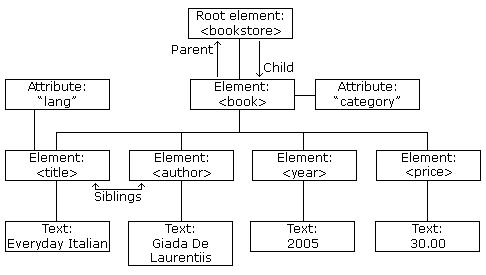
\includegraphics[scale=0.4]{nodetree.jpg}
\vspace{-10pt}
\caption{Tree structure representing an XML file for a bookstore.}
\vspace{-10pt}
\label{fig:exampleimg1}
\end{figure}

\begin{figure}[htb]
\centering
\lstinputlisting[basicstyle=\ttfamily\scriptsize]{xmlexample.xml}
\vspace{-10pt}
\caption{The corresponding XML file for a bookstore.}
\label{fig:xml}
\end{figure}

An example, taken from w3schools.com \cite{w3schoolsxmlexample}, of a basic XML document more clearly shows the structure and formatting used. Figure \ref{fig:exampleimg1} and Figure \ref{fig:xml} show that $<$bookstore$>$ is the root element of the document, and that all $<$book$>$ elements are contained within $<$bookstore$>$. The book element has 4 'children': $<$title$>$, $<$author$>$, $<$year$>$ and $<$price$>$. These children as used to describe and give properties to the associated book. Within this project, the XML files will be set out quite similar, with the full document set up displayed in the design section of this report. 

\subsection{Data Storage}

%mysql - website and book - look for ideas
In order to store and manage the data for each user (I.D, encryption information, messages), MySQL \cite{mysql} will be used. MySQL is the most popular and highly used open source relational database management system (RDBMS). It provides user access to a server which hosts a number of databases. This server can be set up locally on through an external provider. In order to connect, access and edit the database through the developed system, JDBC will be used. 'JDBC is a set of programming APIs that allows easy connection to a wide range of databases (especially relational databases) through Java programs' \cite{jdbcmysql}. JDBC programming involves creating and executing SQL queries or 'statements' and processing the returned ResultSet objects. Statements contain the commands to select or edit particular entries in the database. A full description of the design of the database system in this project will be included in the following chapter. 

\section{Available Applications}

The research completed into the applications for encrypted message transfer that are currently available will now be presented. The two 'non-standard' applications were the only applications that could be found on the google play marketplace \cite{googleplay} through the use of various related search keywords. Most applications that where returned focused on encrypting stored data on the smarphone, as opposed to encrypting messages for sending or receiving, showing that there is a requirement in the market for more secure message communication applications. A full explanation and study of the relevant encryption methods will be displayed in the next section.

\subsection{Short Messaging Service}

The short messaging service is a text messaging service featured on all makes and models of mobile and smart phone. The user enters the recipients mobile telephone number and can send a short message (of only text) to the recipient. These messages are encrypted between the phone and base station however, it is required by law that government enforcement agencies can and should be able to conduct lawful surveillance of SMS messages when required \cite{aresmssafe}. Because of this, unlawful access to SMS messages is possible, by means other than actually breaking the encryption on the messages.

\subsection{Cloak SMS}

Cloak SMS \cite{cloaksms} is an Android application developed by Hamish Medlin. The features of this application are: 

\begin{itemize}
 \item Send and Receive AES Encrypted SMS messages
 \item Threaded Conversations
 \item Application lock
 \item Custom themes
 \item File Encryption
\end{itemize}

Figure \ref{fig:cloaksms} shows the screen used for inputting a message and recipient information. The password is used in the key creation for the cencryption method. The main feature of this application, which is the goal of this research to find out, is that it utilises the AES encryption method. Application locking and file encryption are integrated features which are provided by other applications developed by Hamish and whilst useful in practice, are not relevant to this project. Custom themes and threaded conversations are present for marketability and design as opposed to increasing the security of the application. The cost of this application is £1.00, with a free version available with limited features. Overall the application has generally positive feedback, with an average rating of 4.8/5.

\begin{figure}[htb]
\centering
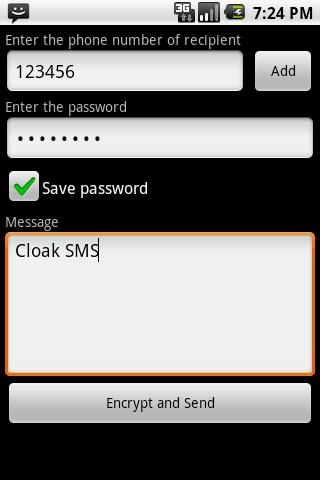
\includegraphics[scale=0.5]{cloaksms.jpg}
\caption{A screen capture of the application in use.}
\vspace{-10pt}
\label{fig:cloaksms}
\end{figure}

\subsection{RSA Cipher Cat}

RSA Cipher Cat is an application developed by Miasoft \cite{rsaciphercat}, which makes use of the RSA public-key encryption scheme. Figure \ref{fig:ciphercat} shows the two main screens of the application, one for encryption (\ref{fig:cat2}) and one for decryption (\ref{fig:cat1}). The disadvantage of this application is that it very basic, as it does not facilitate the sending of the messages, it only performs the actual encryption and decryption, using files given to the application by the user. It is then up to the user to send the encrypted message however they wish. Whilst it does not have the full features of the other applications, it is perfectly appropriate for this project, as it gives an insight into the current state of encrypted message sending applications and an example of cryptography in practice. The application is free to the public, but has a low user review rating of 1/5, submitted by a single user, whilst having between 500-1,000 installs. 

\begin{figure}
        \centering
        \begin{subfigure}[b]{0.45\textwidth}
                \centering
                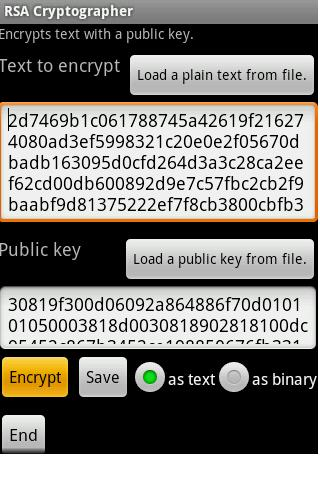
\includegraphics[width=\textwidth]{cat2.jpg}
                \caption{Encrypting a message}
                \label{fig:cat2}
        \end{subfigure}
	\begin{subfigure}[b]{0.45\textwidth}
                \centering
                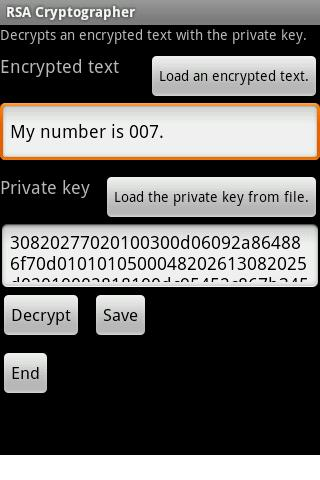
\includegraphics[width=\textwidth]{cat1.jpg}
                \caption{Decrypting a message}
                \label{fig:cat1}
        \end{subfigure}
        \caption{Application usage screen captures}\label{fig:ciphercat}
\end{figure}

\section{Cryptographic Techniques}

\section{Comparison Factors}

As the third section of this project is centred around the analysis and comparison of the various cryptographic schemes implemented through the software development, research was performed in order to discover which factors contribute to how successful or useful the implemented schemes are. Most of the discovered factors were found in the article by Nirav Jobanputra, \textit{et al} \cite{ejeta}. This article studies not only the comparisons of various cryptographic techniques when implemented on a smartphone, but also Bio-information based security solutions such as finger-printing or voice recognition. However, the article was published in 2009 and has therefore the conclusions have lost some relevance due to the multitude of advancements that have been made regarding smartphones. 

That comparison factors that were found that could be used when analysis and concluding the results of this project were:

\begin{itemize}
 \item \textbf{Difficulty of techniques required to break encryption} - Level of various cryptanalytic techniques required to break the encryption. 
 \item \textbf{Battery usage} - Percent of battery usage for the duration of the application completing its required tasks. 
 \item \textbf{Key generation time} - The time it takes to generate the particular key.
 \item \textbf{Encryption and Decryption time} - The time it takes from start to finish to encrypt and decrypt a particular controlled file. 
 \item \textbf{Cryptographic key size} - Size of the key required for the particular cryptographic technique. 
 \item \textbf{Data usage} - Amount of data that is stored by the application and the amount of data that is sent or received. 
 \item \textbf{Application size} - Size of the application once it has been installed on the smartphone. 
 \item \textbf{Number of server connections} - The number of times any sort of data needs to be sent from the server to the phone or the converse.   
\end{itemize}

A combination of these comparison factors will be used to fully compare and contrast all aspects of the cryptographic schemes that will be implemented in this project. 

\appendix
\chapter{Gantt Chart}\label{A}
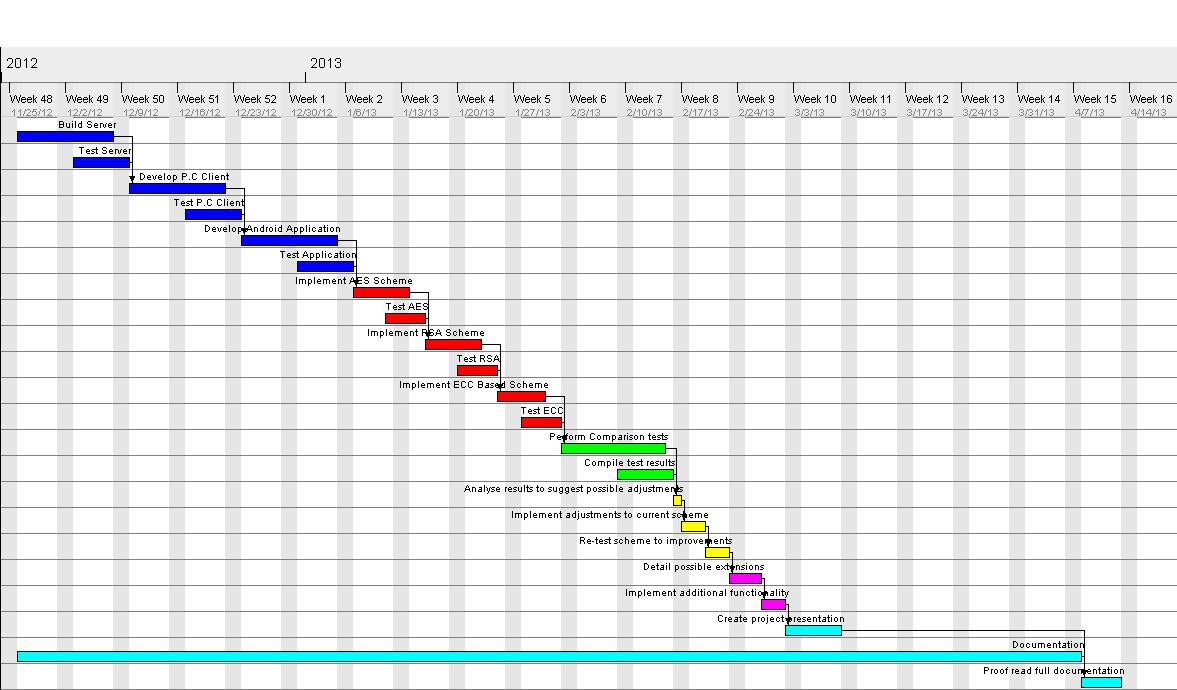
\includegraphics[scale=0.35, angle=270]{ProgReportChart.jpg}

\bibliography{projectbib}

\end{document}          